\documentclass[10pt, a4paper]{article}

\usepackage{ctex}
\usepackage{xeCJK}
\usepackage{caption}
\usepackage{geometry}
\geometry{
    left = 0.6in,
    right = 0.6in,
    top = 0.8in,
    bottom = 1.0in
}
\usepackage{amssymb}
\usepackage{amsbsy}
\usepackage{amsmath}
\usepackage{xcolor}
\usepackage{mathrsfs}
\usepackage{graphicx}
\usepackage{pifont}
\usepackage{tasks}
\settasks{
    label = \Alph*. ,
    label-width = 16pt
}
\pagestyle{empty}

\newcommand{\Title}[3]{
    \begin{center}
        \Large \textbf{中国电子学会 #1~年~#2~月 Scratch~#3级考试}
    \end{center}
}
\newcommand{\TimeAndName}[1]{
    \begin{center}
        考试时间:~#1~ 分钟 \qquad\qquad\qquad\qquad 姓名:\underline{\quad\quad\quad\quad}
    \end{center}
}

\begin{document}
    \Title{2021}{12}{二} % 标题
    \TimeAndName{60} % 考试时间及姓名

    % 单选题
    \vspace{2mm}
    {\noindent\textbf{第一部分、单选题(共 25 题,每题 2 分,共50分.)}}
    \begin{enumerate}
        % 1
        \item 舞台上有 3 个角色,小猫的程序如下图所示,另外两个角色没有程序。点击绿旗,下列选项正确的是?(\qquad)
        
        \begin{minipage}{.32\textwidth}
            \centering
            \begin{minipage}[t]{.6\textwidth}
                \centering
                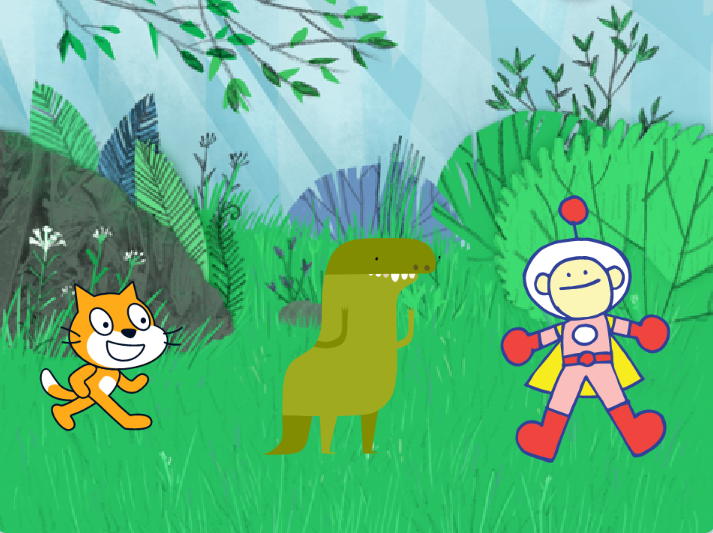
\includegraphics[width=\textwidth]{1-1.png}
            \end{minipage}
            \begin{minipage}[t]{.35\textwidth}
                \centering
                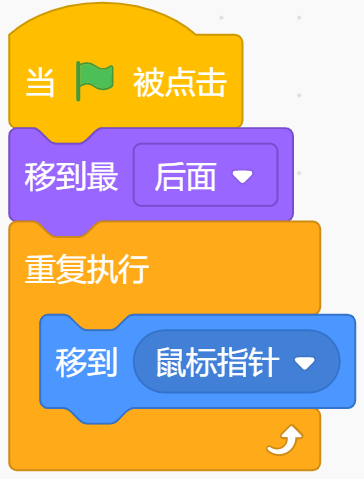
\includegraphics[width=\textwidth]{1-2.png}
            \end{minipage}
        \end{minipage}
        \begin{minipage}{.54\textwidth}
            \begin{tasks}
                \task 小猫随鼠标移动,可能会遮挡其他两个角色
                \task 小猫随鼠标移动,可能会被其他两个角色遮挡
                \task 小猫不会随鼠标移动,更不会被遮挡
                \task 3 个角色会一起随鼠标移动,小猫会遮挡另外两个角色
            \end{tasks}
        \end{minipage}

        % 2
        \item 如下图,点击绿旗,下列选项正确的是?(\qquad)
        \begin{tasks}
            \task 篮球首先出现在1号区域,然后向3号区域滑行,最终停止在3号区域
            \task 篮球首先出现在2号区域,然后向4号区域滑行,最终停止在4号区域
            \task 篮球首先出现在3号区域,然后向1号区域滑行,最终停止在1号区域
            \task 篮球首先出现在4号区域,然后向2号区域滑行,最终停止在2号区域
        \end{tasks}

        \begin{figure}[htbp]
            \centering
            \begin{minipage}[t]{.42\textwidth}
                \centering
                \begin{minipage}[t]{.4\textwidth}
                    \centering
                    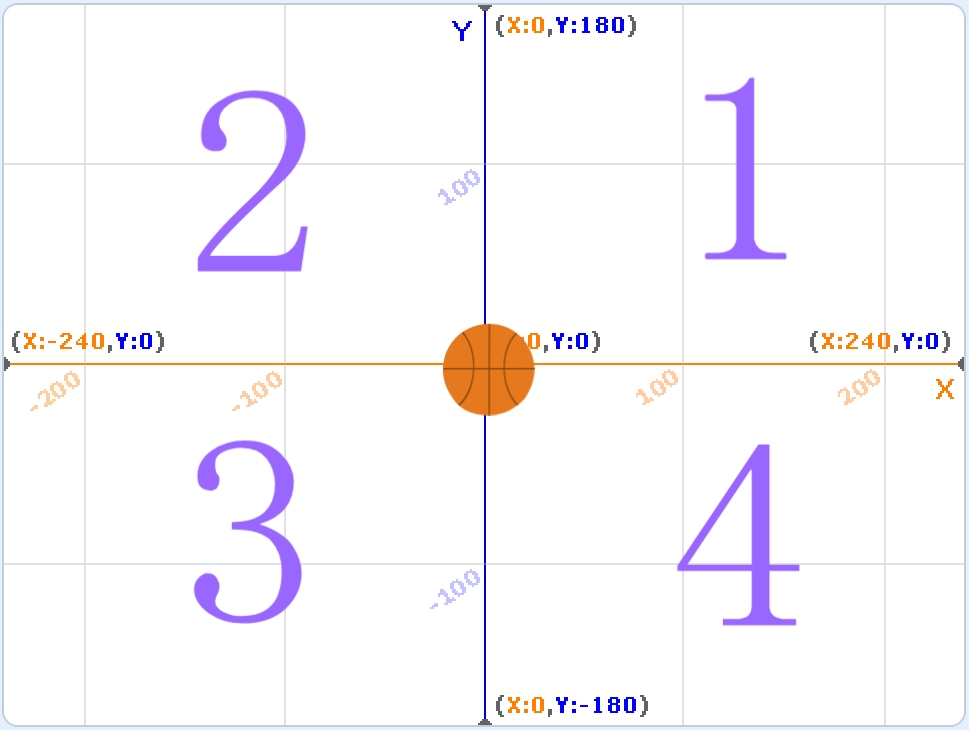
\includegraphics[width=\textwidth]{2-1.png}
                \end{minipage}
                \begin{minipage}[t]{.52\textwidth}
                    \centering
                    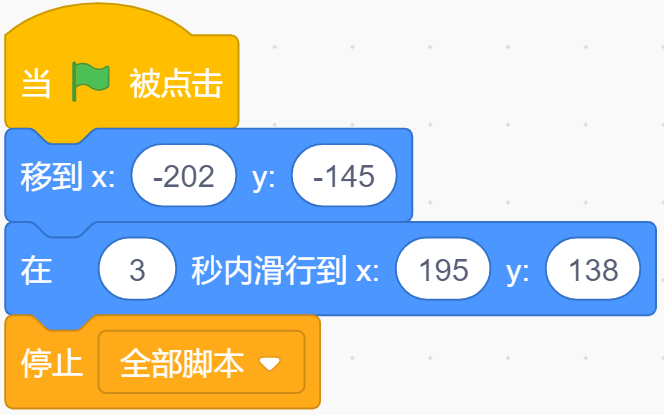
\includegraphics[width=\textwidth]{2-2.png}
                \end{minipage}
                \caption*{第2题}
            \end{minipage}
            \begin{minipage}[t]{.13\textwidth}
                \centering
                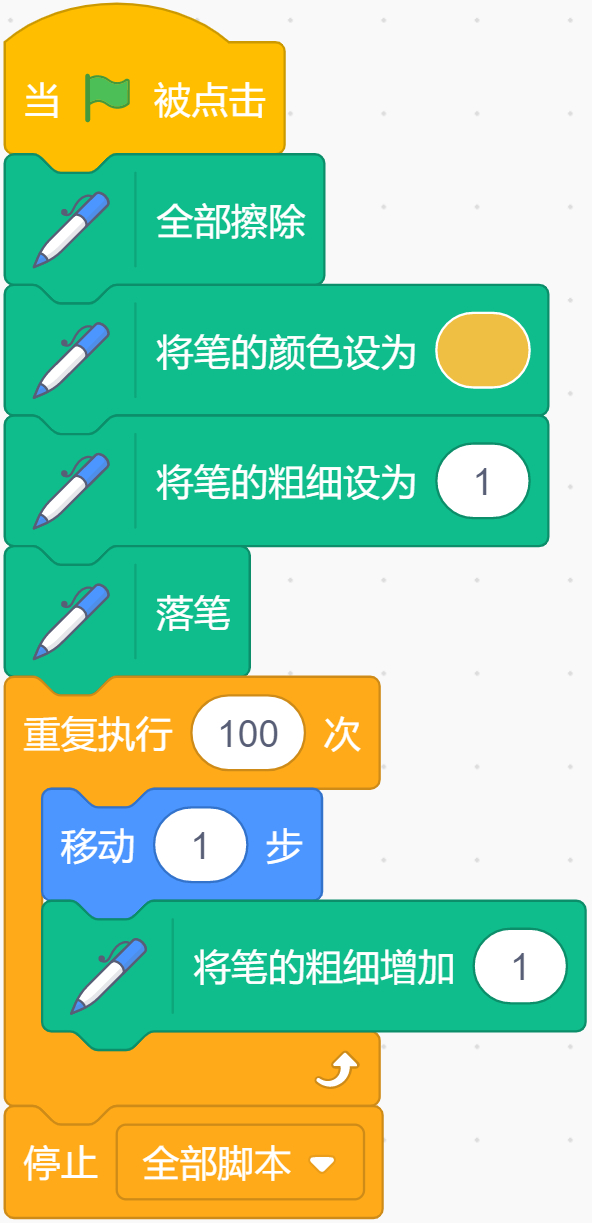
\includegraphics[width=\textwidth]{4.png}
                \caption*{第 4 题}
            \end{minipage}
            \begin{minipage}[t]{.14\textwidth}
                \centering
                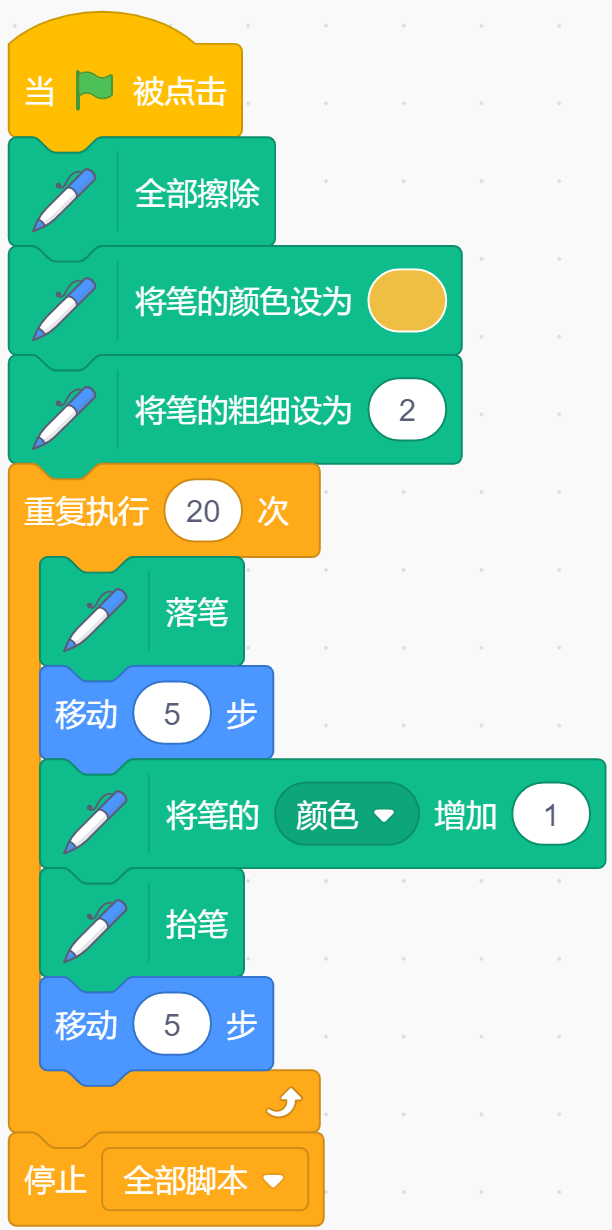
\includegraphics[width=\textwidth]{5.png}
                \caption*{第 5 题}
            \end{minipage}
        \end{figure}

        % 3
        \item 如下图,篮球初始位置在舞台最右侧,大小为100,鼠标指针在舞台最左侧,下列选项错误的是?(\qquad)
        
        \begin{minipage}{.25\textwidth}
            \centering
            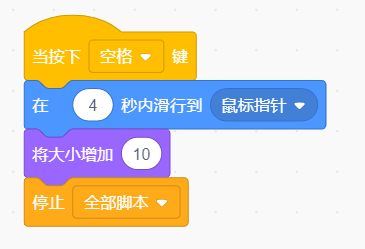
\includegraphics[width=\textwidth]{3.png}
        \end{minipage}
        \begin{minipage}{.64\textwidth}
            \begin{tasks}
                \task 按下空格键,篮球在滑向鼠标指针的过程中不断变大
                \task 按下空格键,篮球在滑到鼠标指针位置后变大
                \task 只有按下空格键后,篮球才会滑行到鼠标指针位置
                \task 按下空格键,篮球会匀速滑动到鼠标的位置
            \end{tasks}
        \end{minipage}

        % 4
        \item 如上图,默认小猫角色,初始位置在舞台中间,面向90方向,点击一次绿旗,下列说法正确的是?(\qquad)
        \begin{tasks}(2)
            \task 程序结束后,看不到任何图形
            \task 会画出一条虚线
            \task 会画出一条实线,且线条粗细一直不变
            \task 随着角色的移动,线条越来越粗
        \end{tasks}

        % 5
        \item 如上图,默认小猫角色,初始位置在舞台中间,面向 90 方向,点击一次绿旗,说法正确的是?(\qquad)
        \begin{tasks}(2)
            \task 会画出一条线条粗细不变的虚线
            \task 会画出一条线条粗细不变的实线
            \task 会画出一条不断变粗的实线
            \task 会画出一条不断变细的虚线
        \end{tasks}

        % 6
        \item 点击绿旗后,鼠标指针移动到 $(-146,89)$ 位置后,鼠标指针不动,下列说法正确的是?(\qquad)
        \begin{tasks}(2)
            \task 角色大小不断变化,一会是100,一会是200
            \task 角色大小为100
            \task 角色大小为200
            \task 角色大小为50
        \end{tasks}

        % 7
        \item 默认小猫角色的程序如下图所示,点击一次绿旗,等待1秒,然后再按方向键,下列说法正确的是?(\qquad)
        \begin{tasks}(2)
            \task 角色会移动到鼠标
            \task 不管按左方向键还是右方向键,角色都不移动
            \task 按左方向键角色向左移动
            \task 按右方向键角色向右移动
        \end{tasks}

        \begin{figure}[htbp]
            \centering
            \begin{minipage}[t]{.15\textwidth}
                \centering
                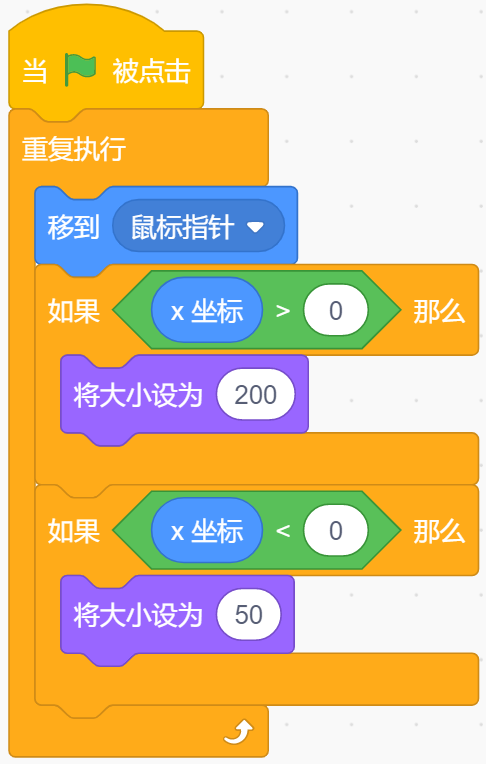
\includegraphics[width=\textwidth]{6.png}
                \caption*{第6题}
            \end{minipage}
            \begin{minipage}[t]{.17\textwidth}
                \centering
                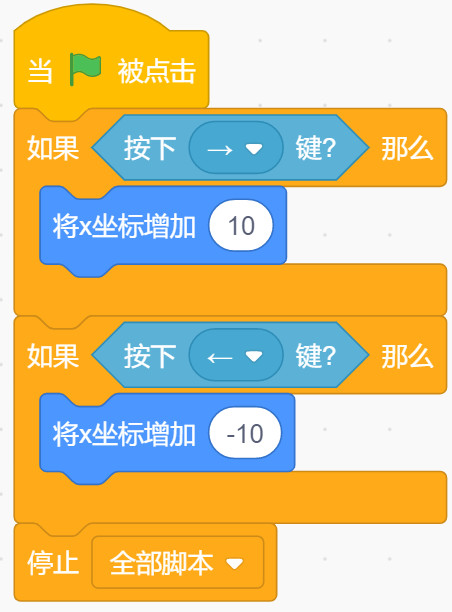
\includegraphics[width=\textwidth]{7.png}
                \caption*{第7题}
            \end{minipage}
            \begin{minipage}[t]{.17\textwidth}
                \centering
                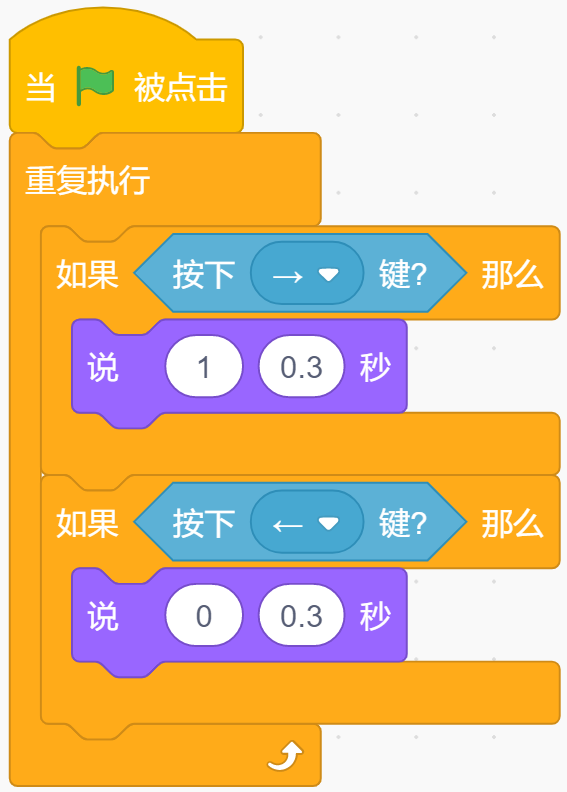
\includegraphics[width=\textwidth]{8.png}
                \caption*{第8题}
            \end{minipage}
            \begin{minipage}[t]{.215\textwidth}
                \centering
                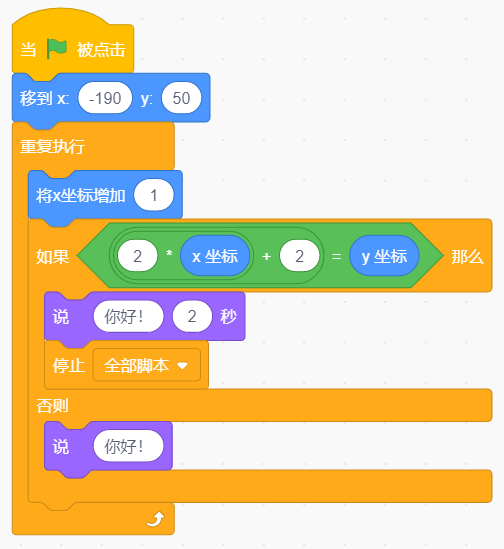
\includegraphics[width=\textwidth]{9.png}
                \caption*{第9题}
            \end{minipage}
            \begin{minipage}[t]{.2\textwidth}
                \centering
                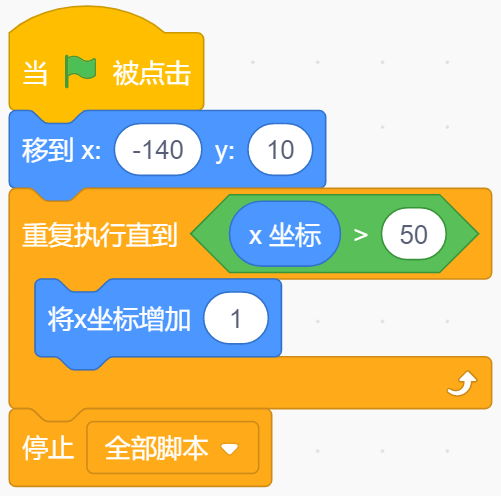
\includegraphics[width=\textwidth]{10.png}
                \caption*{第10题}
            \end{minipage}
        \end{figure}

        % 8
        \item 默认小猫角色的程序如上图所示,以下哪种方向键组合,可以让角色按顺序说出“1”、“0”、“0”、“1”?(\qquad)
        \begin{tasks}(4)
            \task 右、左、左、右
            \task 左、右、右、左
            \task 左、右、左、右
            \task 右、左、右、左
        \end{tasks}

        % 9
        \item 如上图所示,点击绿旗运行程序,当程序停止时,角色的坐标为?(\qquad)
        \begin{tasks}(4)
            \task $(50, -24)$
            \task $(-24, 50)$
            \task $(50, 24)$
            \task $(24, 50)$
        \end{tasks}

        % 10
        \item 如上图所示,点击绿旗执行下列程序,当角色的$x$坐标为多少时,程序停止运行?(\qquad)
        \begin{tasks}(4)
            \task 51
            \task 50
            \task 49
            \task 48
        \end{tasks}

        % 11
        \item 要实现下图中的运行效果,问号处应填写的数值为?(\qquad)
        \begin{tasks}(4)
            \task 5
            \task 6
            \task 7
            \task 8
        \end{tasks}

        \begin{figure}[htbp]
            \centering
            \begin{minipage}[t]{.25\textwidth}
                \centering
                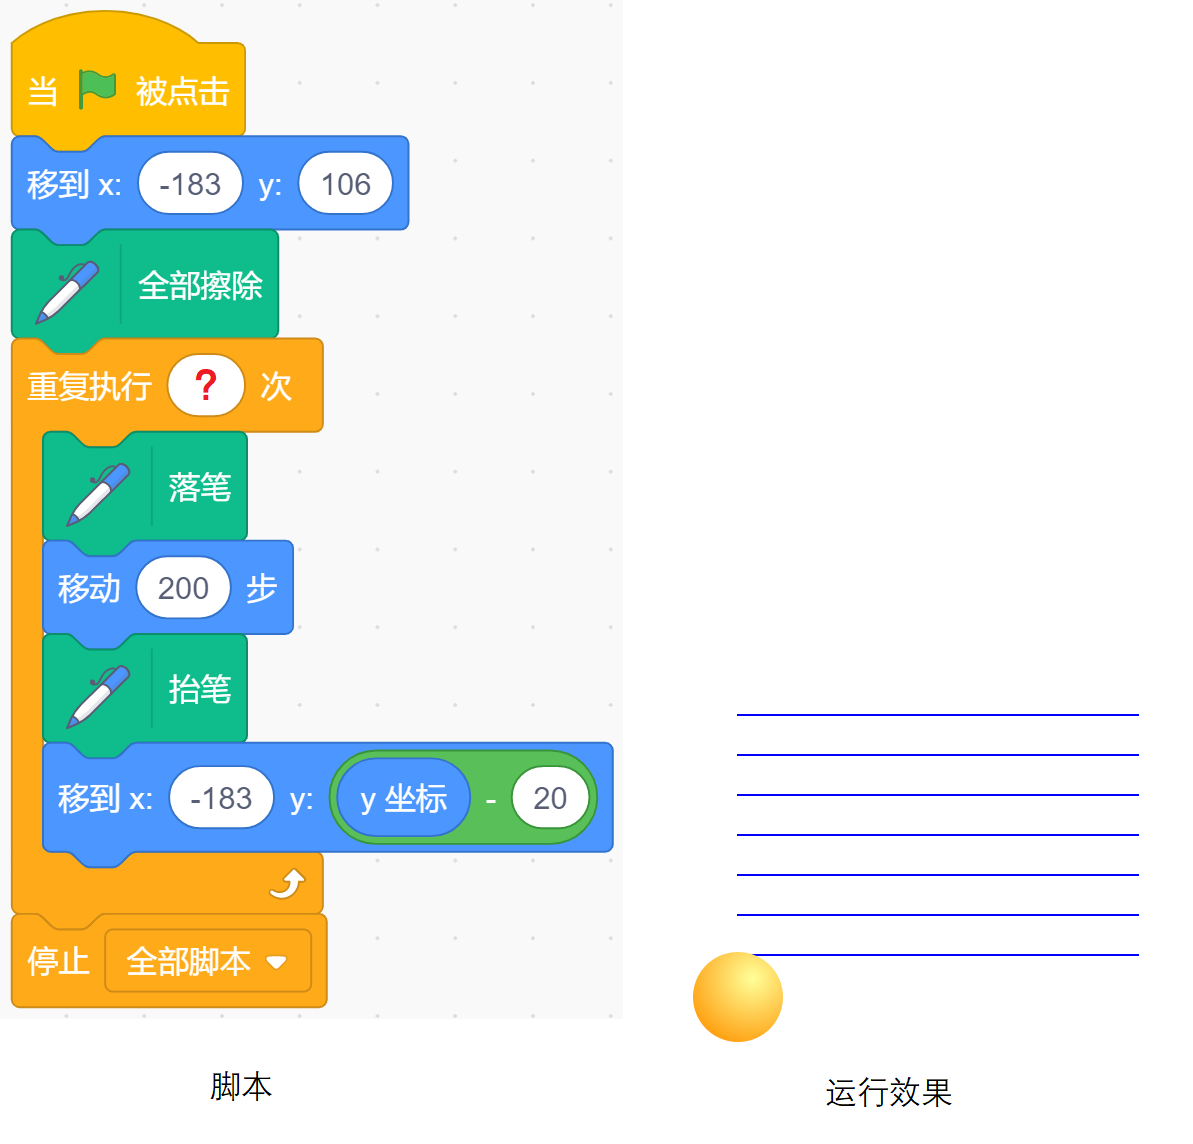
\includegraphics[width=\textwidth]{11-1.png}
                \caption*{第11题}
            \end{minipage}
            \begin{minipage}[t]{.4\textwidth}
                \centering
                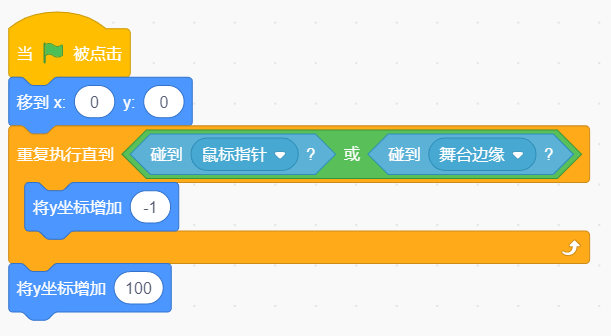
\includegraphics[width=\textwidth]{12.png}
                \caption*{第12题}
            \end{minipage}
        \end{figure}

        % 12
        \item 默认小猫角色,程序如上图所示,点击绿旗,以下说法正确的是?(\qquad)
        \begin{tasks}
            \task 小猫在碰到鼠标或者舞台下边缘前,不断下落,碰到鼠标或者舞台下边缘后,上升100步,程序停止
            \task 小猫在同时碰到鼠标舞台和下边缘前,不断下落,同时碰到鼠标和舞台下边缘后,上升100步,程序停止
            \task 小猫在碰到鼠标或者舞台上边缘前,不断上升,碰到鼠标或者舞台上边缘后,下降100步,程序停止
            \task 小猫在碰到鼠标指针或舞台下边缘后,不断下降,直到看不到小猫,程序停止
        \end{tasks}

        \newpage
        % 13
        \item 默认小猫程序如下图所示,点击绿旗后,下列说法正确的是?(\qquad)
        \begin{tasks}(2)
            \task 程序执行完毕后,小猫的$x$坐标为10
            \task 程序执行完毕后,小猫的$x$坐标为110
            \task 因为$x$坐标不断增加,程序无法停止
            \task 因为$x$坐标不断增加,角色会移出舞台
        \end{tasks}

        % 14
        \item 如下图所示,执行下列程序,以下说法正确的是?(\qquad)
        \begin{tasks}(2)
            \task 按右方向键,角色$x$坐标将被设定为10
            \task 按左方向键,角色$x$坐标将被设定为$-10$
            \task 按上方向键,角色将向上移动
            \task 按下方向键,角色将向上移动
        \end{tasks}

        \begin{figure}[htbp]
            \centering
            \begin{minipage}[t]{.15\textwidth}
                \centering
                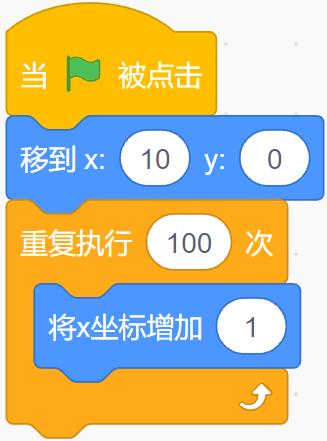
\includegraphics[width=\textwidth]{13.png}
                \caption*{第13题}
            \end{minipage}
            \begin{minipage}[t]{.15\textwidth}
                \centering
                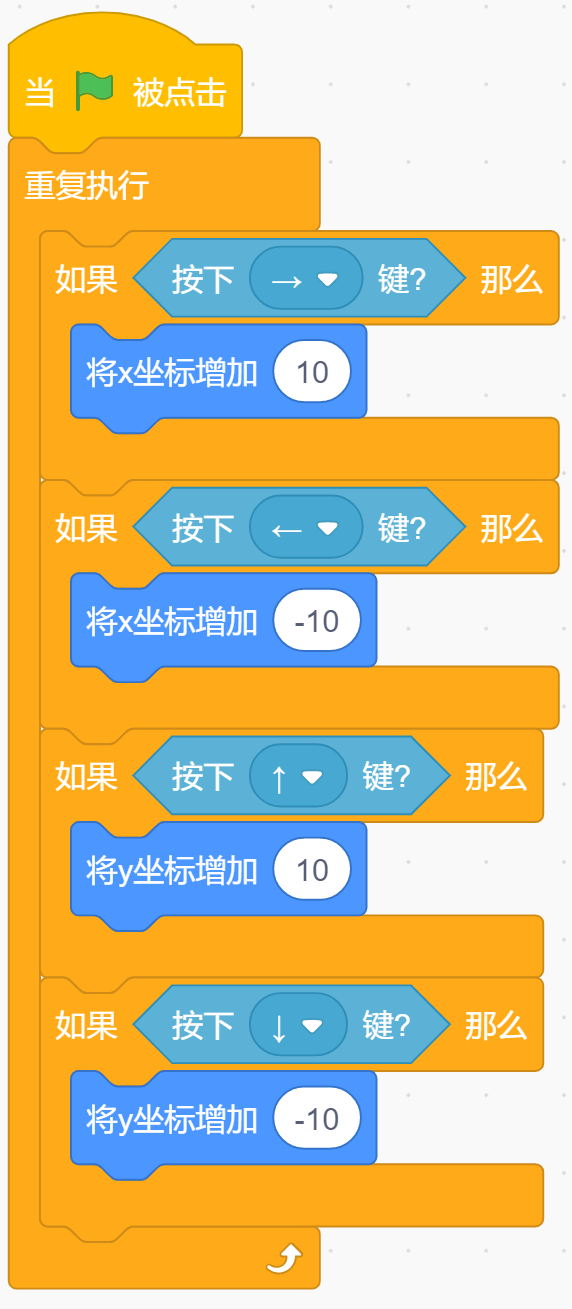
\includegraphics[width=\textwidth]{14.png}
                \caption*{第14题}
            \end{minipage}
            \begin{minipage}[t]{.5\textwidth}
                \centering
                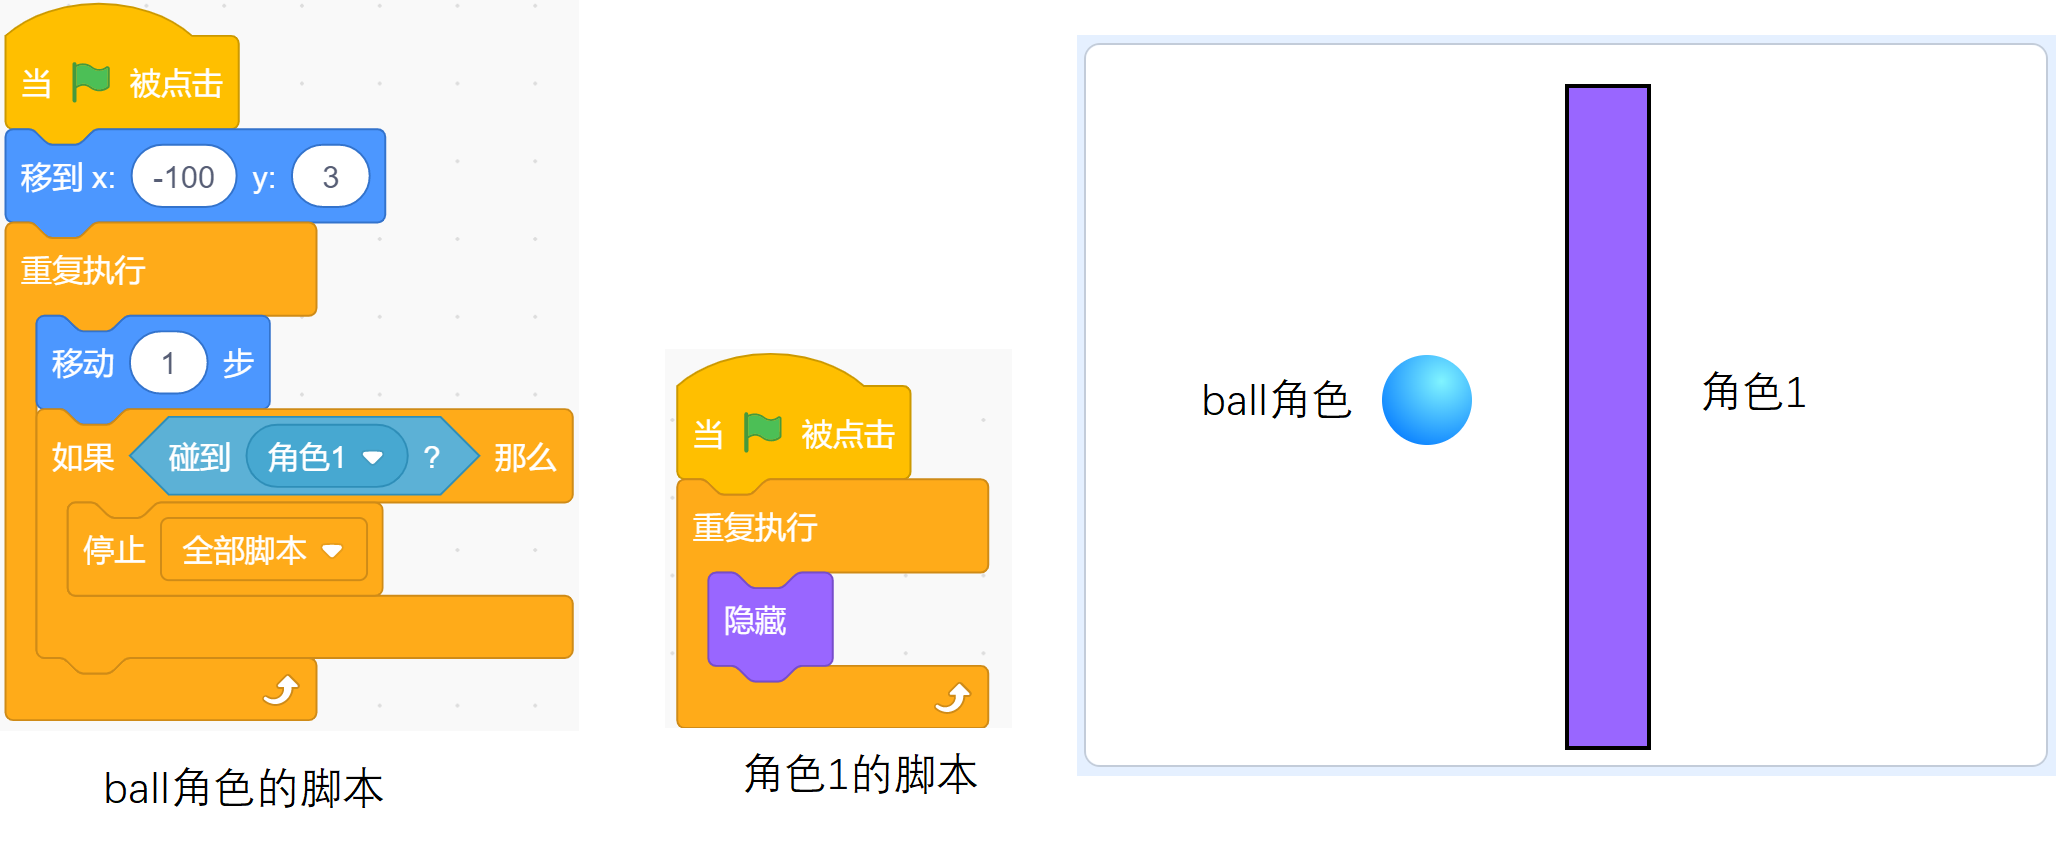
\includegraphics[width=\textwidth]{16-1.png}
                \caption*{第16题}
            \end{minipage}
            \begin{minipage}[t]{.13\textwidth}
                \centering
                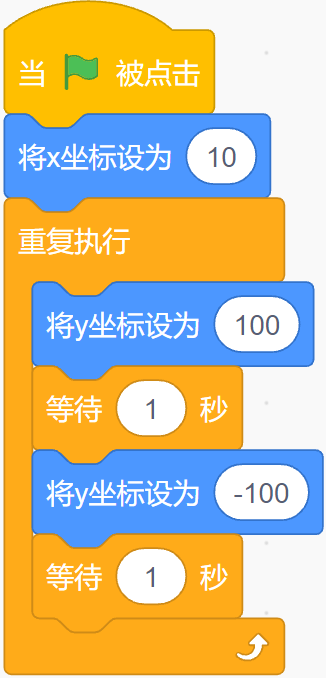
\includegraphics[width=\textwidth]{17.png}
                \caption*{第17题}
            \end{minipage}
        \end{figure}

        % 15
        \item 默认小猫角色和白色背景,点击绿旗,角色静止不动,可能的原因是?(\qquad)
        
        \begin{minipage}{.18\textwidth}
            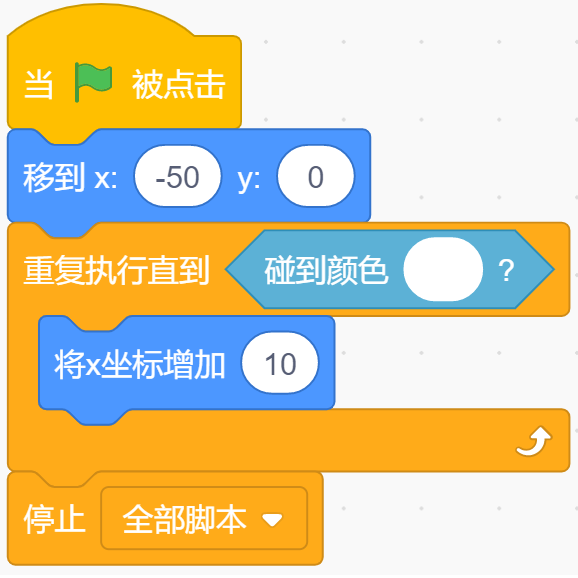
\includegraphics[width=\textwidth]{15.png}
        \end{minipage}
        \begin{minipage}{.6\textwidth}
            \begin{tasks}
                \task 程序中积木“碰到颜色"设置的颜色与背景颜色相同
                \task 角色初始$x$坐标设置错误,应设置为100
                \task 角色初始$y$坐标设置错误,应设置为10
                \task 重复执行内的“将$x$坐标增加10”错误,应设置为“增加100”
            \end{tasks}
        \end{minipage}

        % 16
        \item 如上图所示,ball角色的初始方向为90,点击绿旗,下列说法正确的是?(\qquad)
        \begin{tasks}
            \task 角色1会一直向右移动到舞台右边缘
            \task ball角色会一直向左移动到舞台左边缘
            \task ball角色会向右移动,碰到角色1后,ball停止移动
            \task ball角色会一直向右移动到舞台右边缘
        \end{tasks}

        % 17
        \item 如上图所示,默认小猫角色,运行下列程序后,说法正确的是?(\qquad)
        \begin{tasks}(2)
            \task 小猫在水平方向两个点来回移动
            \task 小猫在垂直方向两个点来回移动
            \task 小猫静止不动
            \task 小猫一直移动,最后移到舞台外面
        \end{tasks}

        % 18
        \item 运行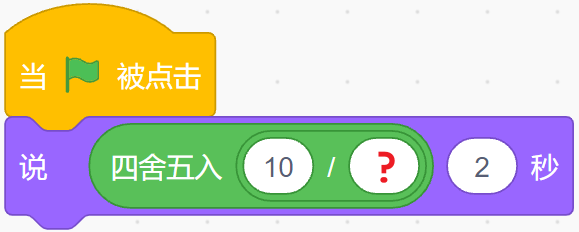
\includegraphics[width=.2\textwidth]{18.png}程序,角色说“3”,问号处是?(\qquad)
        \begin{tasks}(4)
            \task 5
            \task 1
            \task 2
            \task 3
        \end{tasks}

        \newpage
        % 19
        \item 运行下列程序,以下说法正确的是?(\qquad)
        \begin{tasks}
            \task 角色先说“你好”2秒,然后再播声音
            \task 播放声音的同时,角色说“你好”2秒
            \task 先播放声音,等播放完毕后,程序直接结束
            \task 先播放声音,等播放完毕后,角色说“你好”2秒,程序结束
        \end{tasks}

        % 20
        \item 运行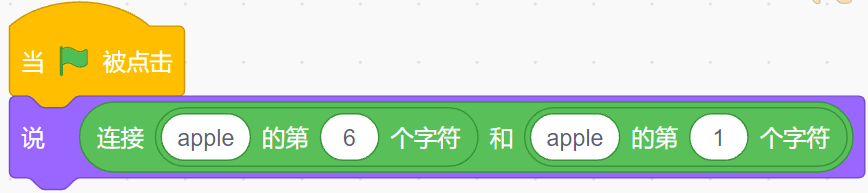
\includegraphics[width=.4\textwidth]{20.png}程序,角色会说出?(\qquad)
        \begin{tasks}(4)
            \task ea
            \task ae
            \task a
            \task 空白
        \end{tasks}

        \begin{figure}[htbp]
            \centering
            \begin{minipage}[t]{.23\textwidth}
                \centering
                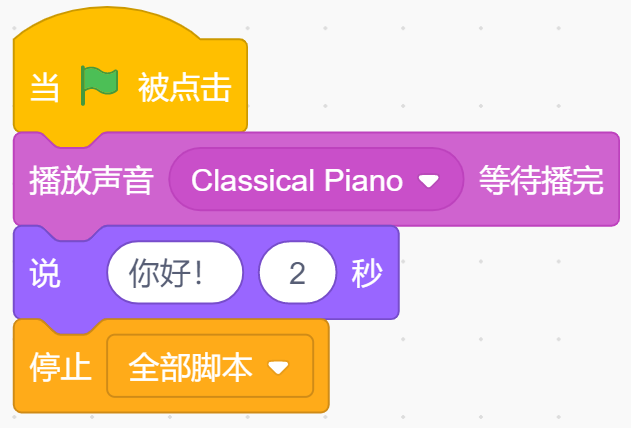
\includegraphics[width=\textwidth]{19.png}
                \caption*{第19题}
            \end{minipage}
            \begin{minipage}[t]{.18\textwidth}
                \centering
                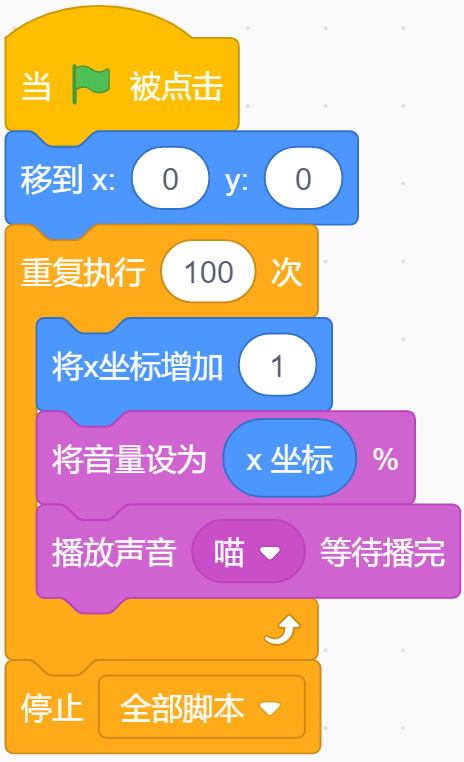
\includegraphics[width=\textwidth]{21.png}
                \caption*{第21题}
            \end{minipage}
            \begin{minipage}[t]{.14\textwidth}
                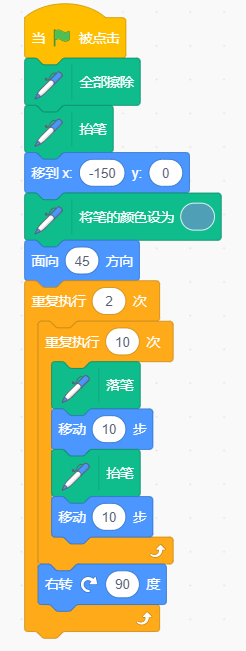
\includegraphics[width=\textwidth]{22.png}
                \caption*{第22题}
            \end{minipage}
            \begin{minipage}[t]{.25\textwidth}
                \centering
                \begin{minipage}[t]{.5\textwidth}
                    \centering
                    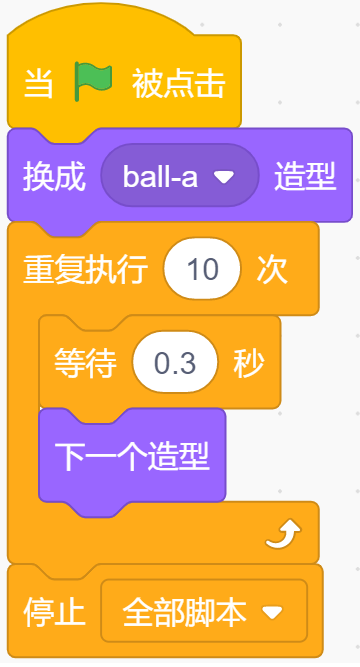
\includegraphics[width=\textwidth]{23-1.png}
                \end{minipage}
                \begin{minipage}[t]{.25\textwidth}
                    \centering
                    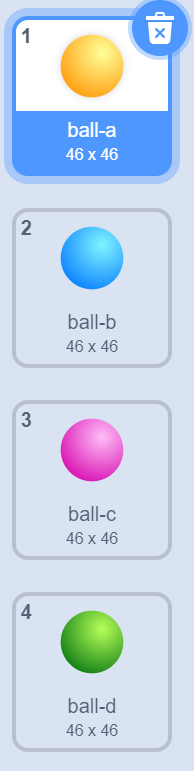
\includegraphics[width=\textwidth]{23-2.png}
                \end{minipage}
                \caption*{第23题}
            \end{minipage}
        \end{figure}

        % 21
        \item 默认小猫角色,初始方向90,点击绿旗,下列说法正确的是?(\qquad)
        \begin{tasks}
            \task 随着小猫向右移动,音量越来越小,程序停止后,$x$坐标为100
            \task 随着小猫向右移动,音量越来越大,程序停止后,音量为100
            \task 随着小猫向左移动,音量越来越大,程序停止后,$x$坐标为100
            \task 随着小猫向左移动,叫声越来越小,程序停止后,音量为100
        \end{tasks}

        % 22
        \item 如上图所示,运行程序后,画出的图形是?(\qquad)
        \begin{tasks}(4)
            \task 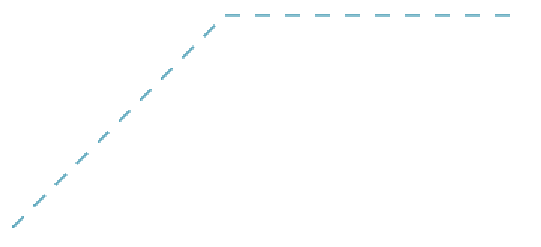
\includegraphics[width=.1\textwidth]{22a.png}
            \task 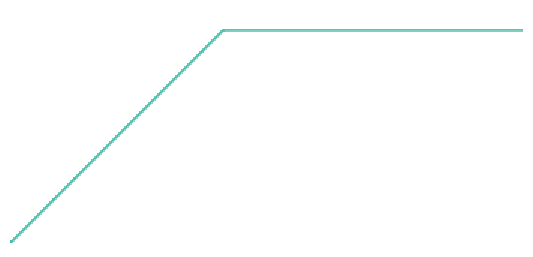
\includegraphics[width=.1\textwidth]{22b.png}
            \task 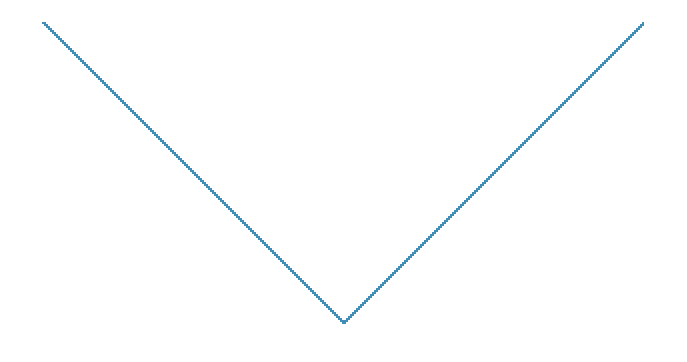
\includegraphics[width=.1\textwidth]{22c.png}
            \task 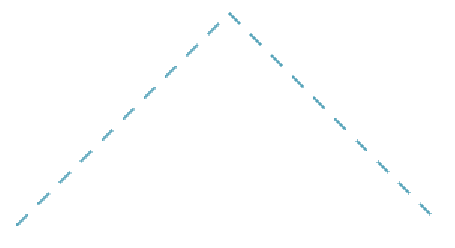
\includegraphics[width=.1\textwidth]{22d.png}
        \end{tasks}

        % 23
        \item 如上图,点击绿旗,角色的造型为?(\qquad)
        \begin{tasks}(4)
            \task 造型ball-a
            \task 造型ball-b
            \task 造型ball-c
            \task 造型ball-d
        \end{tasks}

        % 24
        \item 小猫和它的朋友狐狸一起制作了一种加密算法,加密方法如下:
        \begin{enumerate}
            \item[(1)] 小猫把一句话的顺序颠倒过来,例如“ABCDEF” $\to$ "FEDCBA"
            \item[(2)] 狐狸把第一个字母移到末尾,把其他字母往左边平移,例如“ABCDEF" $\to$ "BCDEFA"
        \end{enumerate}
        狐狸把第一个字母移到末尾,把其他字母往左边平移,例如“ABCDEF" $\to$ "BCDEFA"?(\qquad)
        \begin{tasks}(4)
            \task TIECQ
            \task IECQT
            \task CEITQ
            \task QTIEC
        \end{tasks}

        \newpage
        % 25
        \item 执行下列程序,绘制出正六边形,“甲”、“乙”两个位置的值是多少?(\qquad)
        \begin{tasks}(4)
            \task 甲:3,乙:120
            \task 甲:4,乙:90
            \task 甲:5,乙:72
            \task 甲:6,乙:60
        \end{tasks}
    \end{enumerate}

    \begin{figure}[htbp]
        \centering
        \begin{minipage}[t]{.11\textwidth}
            \centering
            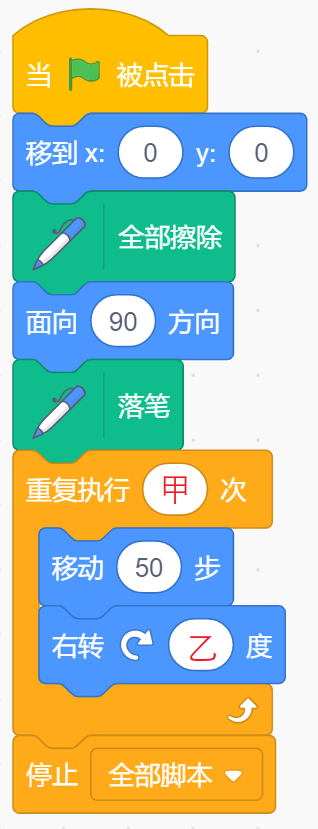
\includegraphics[width=\textwidth]{25.png}
            \caption*{第25题}
        \end{minipage}
        \begin{minipage}[t]{.3\textwidth}
            \centering
            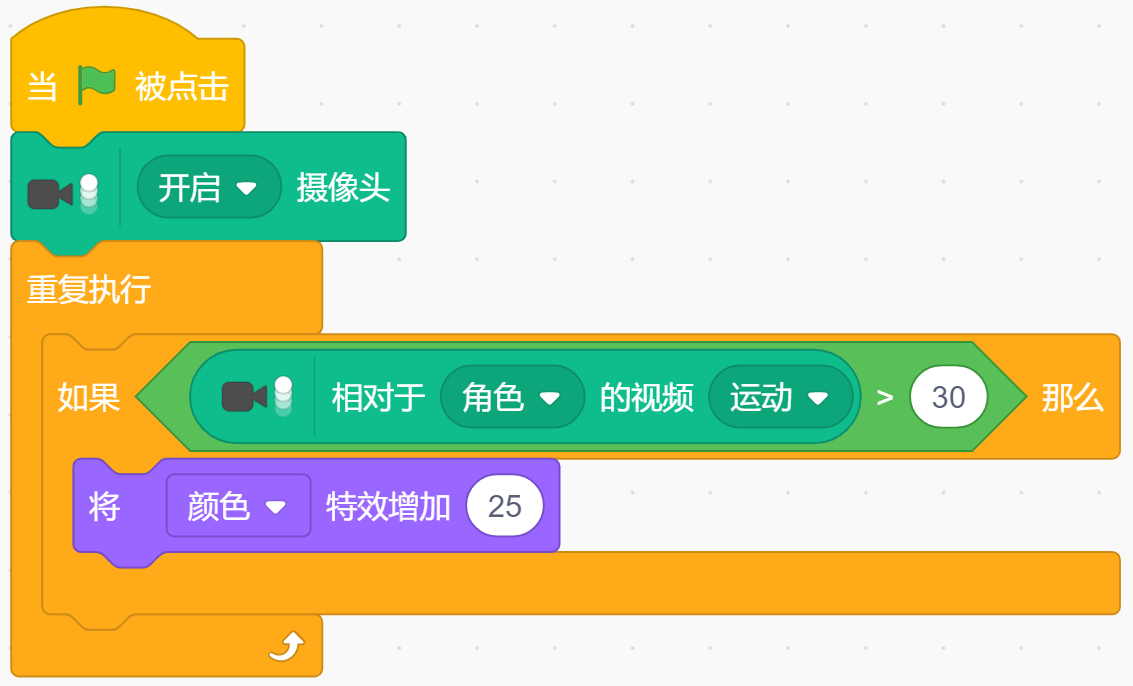
\includegraphics[width=\textwidth]{26.png}
            \caption*{第26题}
        \end{minipage}
        \begin{minipage}[t]{.18\textwidth}
            \centering
            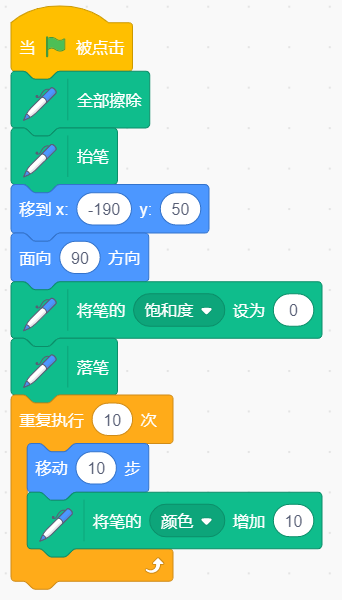
\includegraphics[width=\textwidth]{27.png}
            \caption*{第27题}
        \end{minipage}
        \begin{minipage}[t]{.33\textwidth}
            \centering
            \begin{minipage}[t]{.55\textwidth}
                \centering
                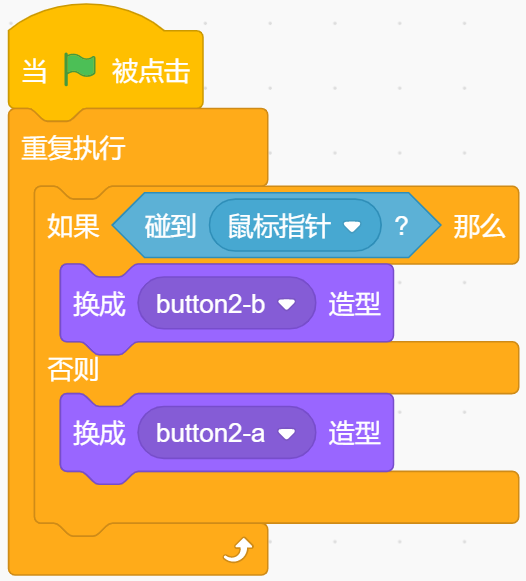
\includegraphics[width=\textwidth]{28-2.png}
            \end{minipage}
            \begin{minipage}[t]{.33\textwidth}
                \centering
                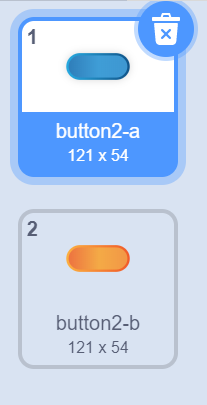
\includegraphics[width=\textwidth]{28-1.png}
            \end{minipage}
            \caption*{第28题}
        \end{minipage}
    \end{figure}

    % 判断题
    {\noindent\textbf{第二部分、判断题(共 10 题,每题 2 分,共20分.)}}
    \begin{enumerate}
        \setcounter{enumi}{25}
        % 26
        \item 执行如上图程序,摄像头前没有物体运动时,角色的颜色不会改变. (\qquad)

        % 27
        \item 如上图,默认小猫角色,点击绿旗,能画出一条颜色不断变化的直线. (\qquad)

        % 28
        \item 如上图,点击绿旗,当鼠标指针放在角色的中间位置时,角色会切换成button2-a造型. (\qquad)
  
        %29
        \item 默认小猫角色,点击绿旗后,每次点击小猫,小猫都会说“你好”2秒. (\qquad)
        
        %30
        \item 执行下列程序,角色的坐标为$(20, 40)$. (\qquad)
        
        %31
        \item 执行下列左图的程序,画出的是右图的图形. (\qquad)
        
        %32
        \item 执行下列程序,角色每碰到一次舞台边缘,就会变换一次造型. (\qquad)
        
        \begin{figure}[htbp]
            \centering
            \begin{minipage}[t]{.25\textwidth}
                \centering
                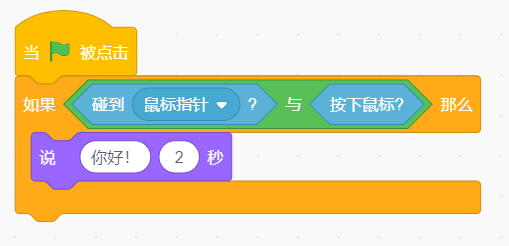
\includegraphics[width=\textwidth]{29.png}
                \caption*{第29题}
            \end{minipage}
            \begin{minipage}[t]{.12\textwidth}
                \centering
                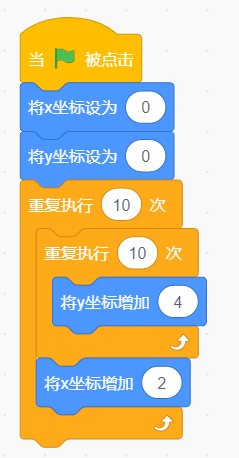
\includegraphics[width=\textwidth]{30.png}
                \caption*{第30题}
            \end{minipage}
            \begin{minipage}[t]{.2\textwidth}
                \centering
                \begin{minipage}[t]{.56\textwidth}
                    \centering
                    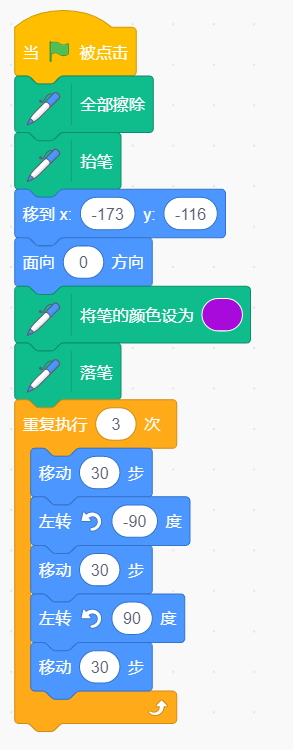
\includegraphics[width=\textwidth]{31-1.png}
                \end{minipage}
                \begin{minipage}[t]{.4\textwidth}
                    \centering
                    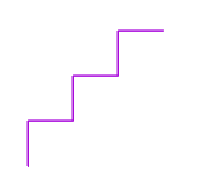
\includegraphics[width=\textwidth]{31-2.png}
                \end{minipage}
                \caption*{第31题}
            \end{minipage}
            \begin{minipage}[t]{.2\textwidth}
                \centering
                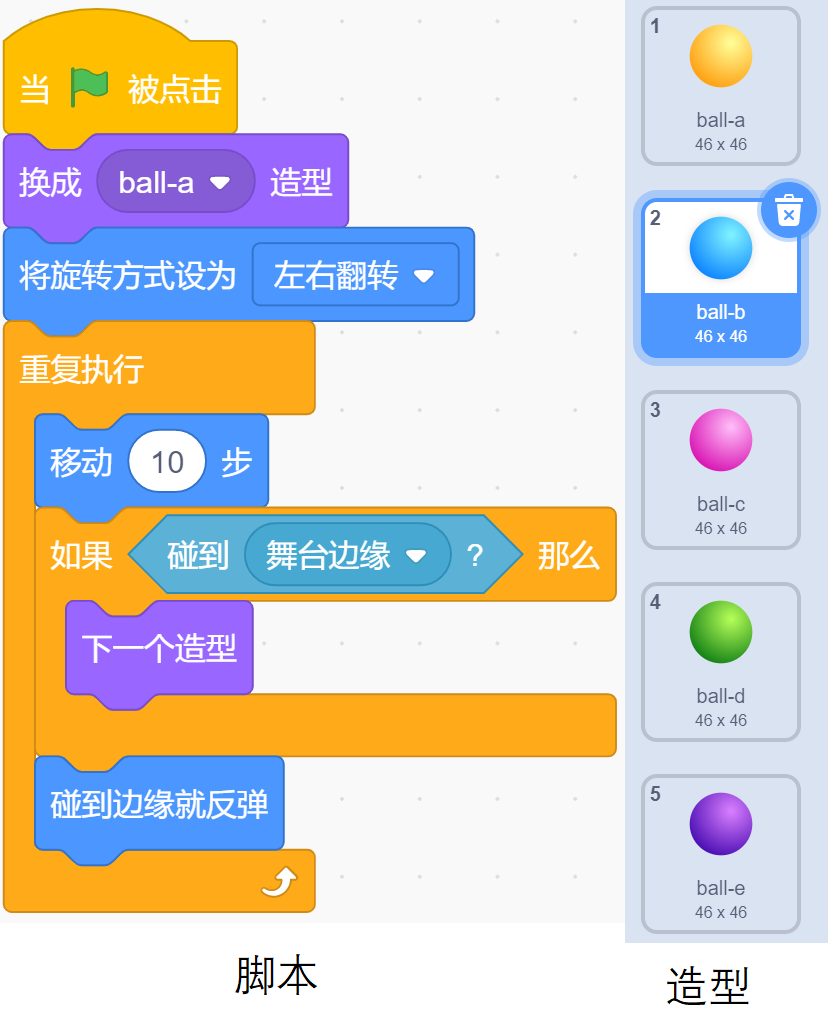
\includegraphics[width=\textwidth]{32-1.png}
                \caption*{第32题}
            \end{minipage}
            \begin{minipage}[t]{.15\textwidth}
                \centering
                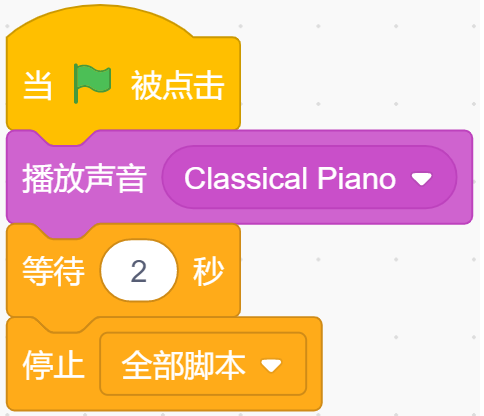
\includegraphics[width=\textwidth]{33.png}
                \caption*{第33题}
            \end{minipage}
        \end{figure}

        %33
        \item 声音Calssical Piano长7.19秒,执行上图程序能将音乐完整播放 .(\qquad)
        
        %34
        \item 无法找到如图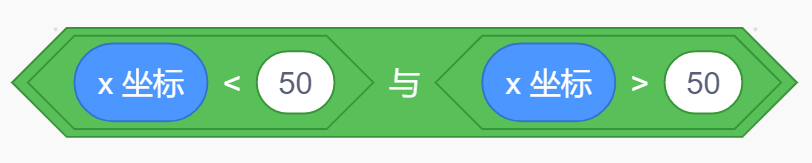
\includegraphics[width=.25\textwidth]{34.png}条件的$x$坐标.(\qquad)
        
        \newpage
        %35
        \item 动漫人物大聚会,喜羊羊要跟五个朋友去打招呼:黑猫警长、唐老鸭、海贼王、皮卡丘和蓝猫,规则如下:
        \begin{enumerate}
            \item[(1)] 跟皮卡丘打招呼前,必须先跟黑猫警长打招呼
            \item[(2)] 跟唐老鸭打招呼前,必须先跟蓝猫打招呼
            \item[(3)] 跟海贼王打招呼前,必须先跟唐老鸭和皮卡丘打招呼
            \item[(4)] 跟黑猫警长打招呼前,必须先跟唐老鸭和蓝猫打招呼
        \end{enumerate}
        如果第一个打招呼的是蓝猫,那么最后打招呼的是海贼王(\qquad)
    \end{enumerate}

    {\noindent \textbf{第三部分、编程题(共 2 题,共30分.)}}
    \begin{enumerate}
        \setcounter{enumi}{35}
        
        % 36
        \item 消灭蝙蝠:
        \begin{figure}[htbp]
            \centering
            \begin{minipage}{.6\textwidth}
                1. 准备工作
                \begin{tasks}[label = (\arabic*)]
                    \task 选择背景Night City;
                    \task 选择角色Bat、Ripley。
                \end{tasks}
                2. 功能实现
                \begin{tasks}[label = (\arabic*)]
                    \task 初始的背景为Night City,Bat的初始位置在舞台上方,Ripley初始位置在舞台下方;
                    \task 点击绿旗,Bat调整方向后,在整个舞台上飞来飞去,飞行过程中不断煽动翅膀;
                    \task Ripley随着鼠标移动,碰到Bat,Bat发出声音owl,Bat移到舞台随机位置。
                \end{tasks}
            \end{minipage}
            \begin{minipage}{.3\textwidth}
                \centering
                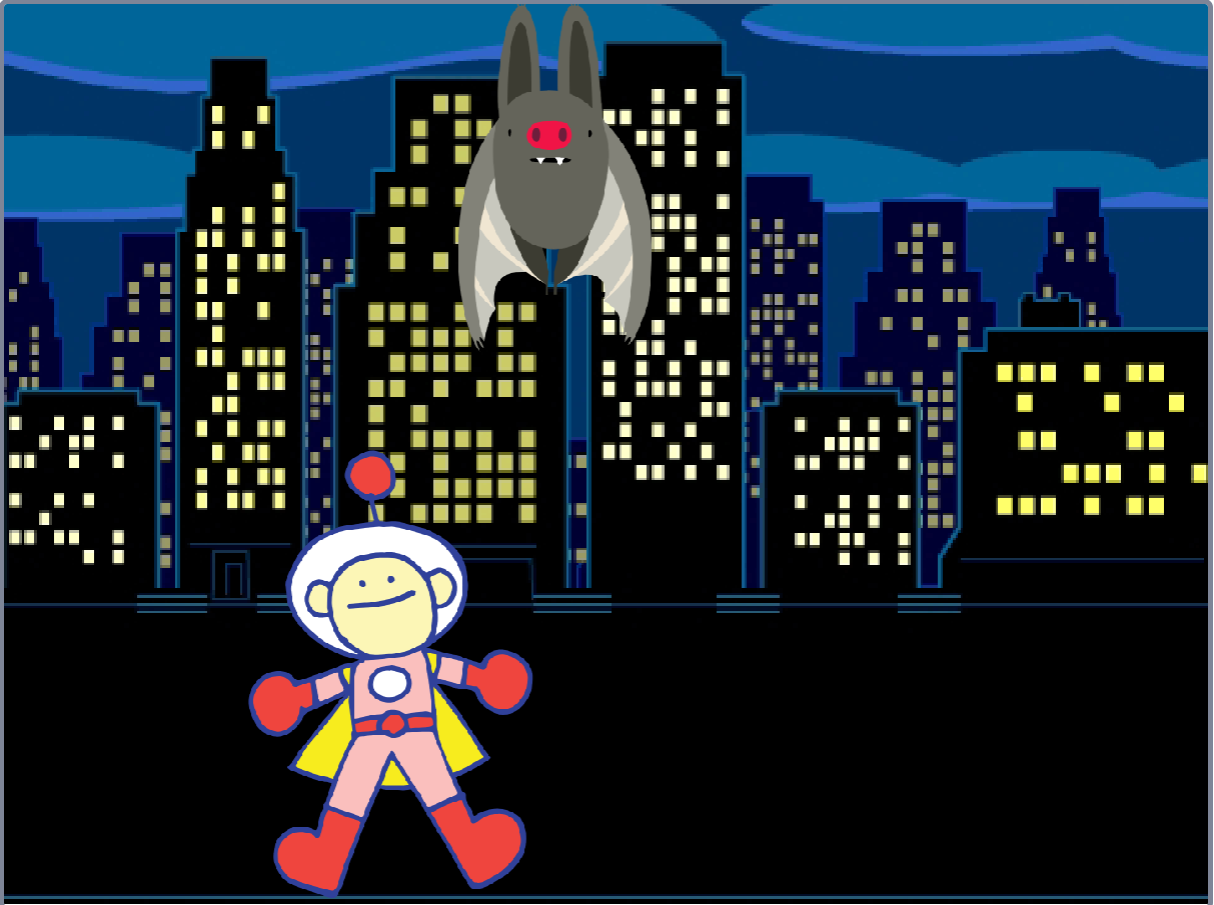
\includegraphics[width=\textwidth]{36.png}
            \end{minipage}
        \end{figure}

        %37
        \item 绘制图形:
        \begin{figure}[htbp]
            \centering
            \begin{minipage}{.6\textwidth}
                1. 准备工作
                \begin{tasks}[label = (\arabic*)]
                    \task 选择背景Blue Sky 2;
                    \task 选择角色箭头。
                \end{tasks}
                2. 功能实现
                \begin{tasks}[label = (\arabic*)]
                    \task 箭头初始位置在舞台中心;
                    \task 大的多边形的边长为50,线条粗细5,线条颜色蓝色;
                    \task 小多边形的边长为10;
                    \task 绘制如下图所示图形;
                    \task 绘制结束后角色隐藏。 
                \end{tasks}
            \end{minipage}
            \begin{minipage}{.3\textwidth}
                \centering
                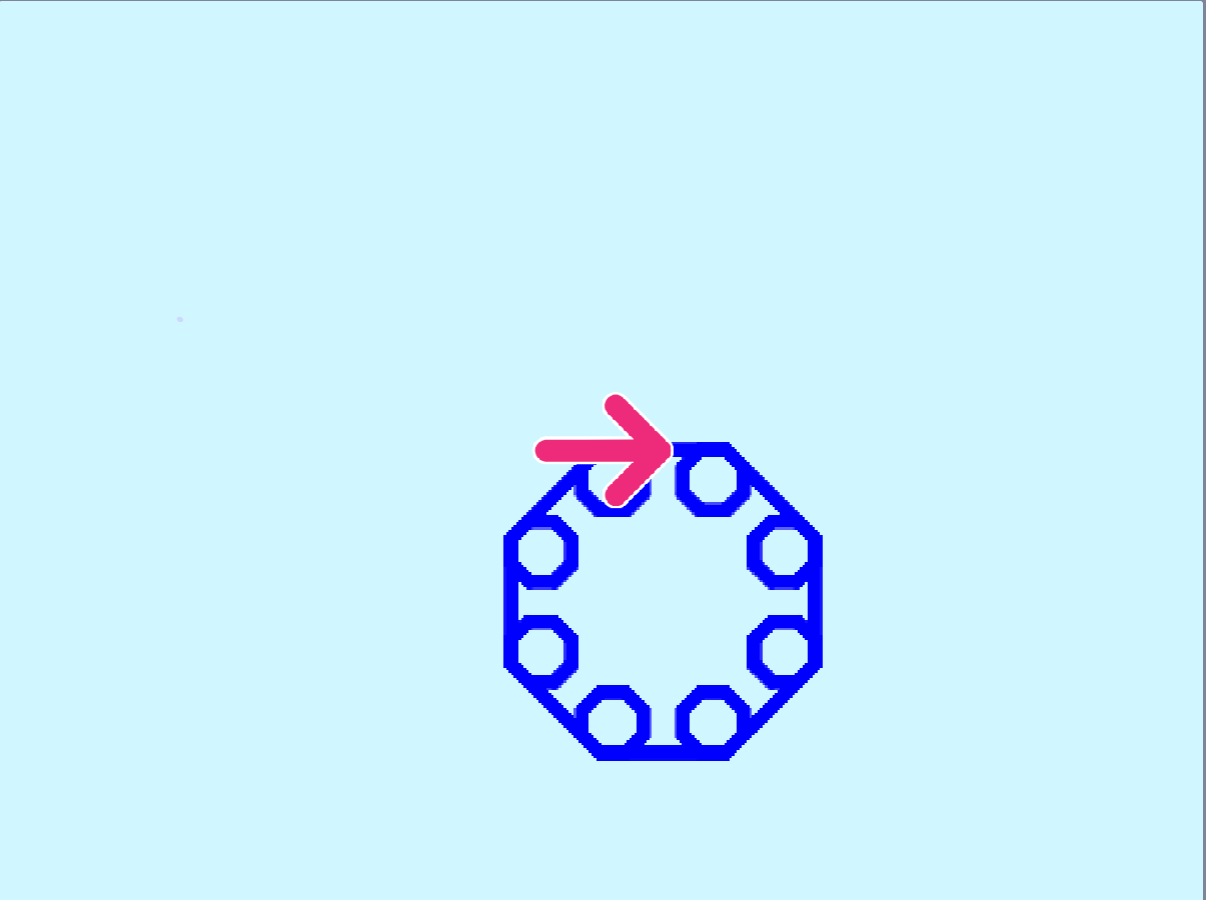
\includegraphics[width=\textwidth]{37.png}
            \end{minipage}
        \end{figure}
    \end{enumerate}
\end{document}